\documentclass[11pt]{article}
%\usepackage[a3paper]{geometry}
%\usepackage[]{babel}
\usepackage[utf8]{inputenc}
\usepackage[T1]{fontenc}
\usepackage{fancyhdr}
\usepackage{graphicx}
\usepackage{amsmath}
\usepackage{amsfonts}
\usepackage{enumerate}
\PassOptionsToPackage{hyphens}{url}\usepackage{hyperref}
\usepackage {tikz}
\usetikzlibrary {positioning,fit,matrix,chains,calc,shapes.multipart,arrows,decorations.pathreplacing,shapes.arrows,chains,positioning}
\newlength\myht
\settoheight{\myht}{$n-2$}
%\usepackage{pgf}
%\usepgfplotslibrary{units}


\topmargin=0cm \oddsidemargin=0cm \evensidemargin=0cm \textheight=21cm
\textwidth=16cm \headheight=15pt \footskip=35pt

%\topmargin=0cm \oddsidemargin=0cm \evensidemargin=0cm \textheight=35cm
%\textwidth=25cm \headheight=15pt \footskip=35pt

\pagestyle{fancyplain}
\fancyhead{} % clear all header fields
\lhead{Enseirb-Matmeca M2 2021-2022}
\rhead{Quickly Différences Finies 2D}
\fancyfoot{} % clear all footer fields
\cfoot{\thepage}

\begin{document}

%headers
\begin{center}
{\bf \Large Quickly Différences Finies 2D } \\ 
N. Barral (\href{mailto:nicolas.barral@enseirb-matmeca.fr}{nicolas.barral@enseirb-matmeca.fr})
\end{center}
\hrule
\vspace*{1cm}

% beginning of the content


\begin{figure}[!ht]
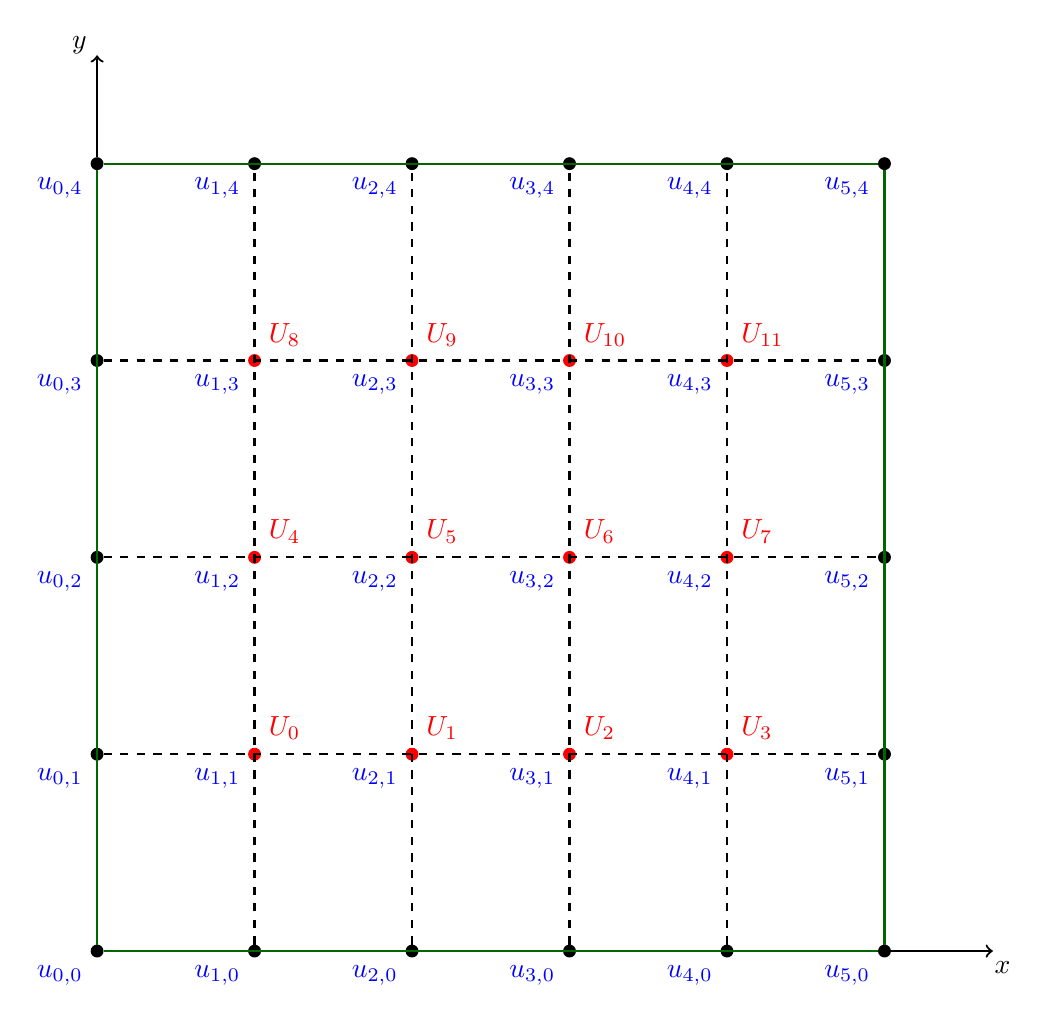
\begin{tikzpicture}[scale=1, , every node/.style={transform shape},
vertex/.style={circle, draw, fill, color=black, inner sep=1.5pt}]

\node[vertex, label={[blue]below left:$u_{0,0}$}] (1) at   (00.,00.0)     {};
\node[vertex, label={[blue]below left:$u_{0,1}$}] (2) at   (00.,02.5)     {};
\node[vertex, label={[blue]below left:$u_{0,2}$}] (3) at   (00.,05.0)     {};
\node[vertex, label={[blue]below left:$u_{0,3}$}] (4) at   (00.,07.5)     {};
\node[vertex, label={[blue]below left:$u_{0,4}$}] (5) at   (00.,10.0)     {};
\node[]       (5bis) at(00.,11.5)     {};
\node[vertex, label={[blue]below left:$u_{1,0}$}] (6) at   (02.,00.0)     {};
\node[vertex, red, label={[blue]below left:$u_{1,1}$}, label={[red]above right:$U_{0}$}] (7) at   (02.,02.5)     {};
\node[vertex, red, label={[blue]below left:$u_{1,2}$}, label={[red]above right:$U_{4}$}] (8) at   (02.,05.0)     {};
\node[vertex, red, label={[blue]below left:$u_{1,3}$}, label={[red]above right:$U_{8}$}] (9) at   (02.,07.5)     {};
\node[vertex, label={[blue]below left:$u_{1,4}$}] (10) at  (02.,10.0)     {};
\node[vertex, label={[blue]below left:$u_{2,0}$}] (11) at  (04.,00.0)     {};
\node[vertex, red, label={[blue]below left:$u_{2,1}$}, label={[red]above right:$U_{1}$}] (12) at  (04.,02.5)     {};
\node[vertex, red, label={[blue]below left:$u_{2,2}$}, label={[red]above right:$U_{5}$}] (13) at  (04.,05.0)     {};
\node[vertex, red, label={[blue]below left:$u_{2,3}$}, label={[red]above right:$U_{9}$}] (14) at  (04.,07.5)     {};
\node[vertex, label={[blue]below left:$u_{2,4}$}] (15) at  (04.,10.0)     {};
\node[vertex, label={[blue]below left:$u_{3,0}$}] (16) at  (06.,00.0)     {};
\node[vertex, red, label={[blue]below left:$u_{3,1}$}, label={[red]above right:$U_{2}$}] (17) at  (06.,02.5)     {};
\node[vertex, red, label={[blue]below left:$u_{3,2}$}, label={[red]above right:$U_{6}$}] (18) at  (06.,05.0)     {};
\node[vertex, red, label={[blue]below left:$u_{3,3}$}, label={[red]above right:$U_{10}$}] (19) at  (06.,07.5)     {};
\node[vertex, label={[blue]below left:$u_{3,4}$}] (20) at  (06.,10.0)     {};
\node[vertex, label={[blue]below left:$u_{4,0}$}] (21) at  (08.,00.0)     {};
\node[vertex, red, label={[blue]below left:$u_{4,1}$}, label={[red]above right:$U_{3}$}] (22) at  (08.,02.5)     {};
\node[vertex, red, label={[blue]below left:$u_{4,2}$}, label={[red]above right:$U_{7}$}] (23) at  (08.,05.0)     {};
\node[vertex, red, label={[blue]below left:$u_{4,3}$}, label={[red]above right:$U_{11}$}] (24) at  (08.,07.5)     {};
\node[vertex, label={[blue]below left:$u_{4,4}$}] (25) at  (08.,10.0)     {};
\node[vertex, label={[blue]below left:$u_{5,0}$}] (26) at  (10.,00.0)     {};
\node[]       (26bis) at(11.5,0.)     {};
\node[vertex, label={[blue]below left:$u_{5,1}$}] (27) at  (10.,02.5)     {};
\node[vertex, label={[blue]below left:$u_{5,2}$}] (28) at  (10.,05.0)     {};
\node[vertex, label={[blue]below left:$u_{5,3}$}] (29) at  (10.,07.5)     {};
\node[vertex, label={[blue]below left:$u_{5,4}$}] (30) at  (10.,10.0)     {};

\draw[thick, black!60!green] (1) -- (5);
\draw[thick, ->] (5) -- (5bis) node[left]{$y$};
\draw[thick, dashed] (6) -- (10);
\draw[thick, dashed] (11) -- (15);
\draw[thick, dashed] (16) -- (20);
\draw[thick, dashed] (21) -- (25);
\draw[thick, black!60!green] (26) -- (30);
\draw[thick, black!60!green] (1) -- (26);
\draw[thick, ->] (26) -- (26bis) node[below]{$x$};
\draw[thick, dashed] (2) -- (27);
\draw[thick, dashed] (3) -- (28);
\draw[thick, dashed] (4) -- (29);
\draw[thick, black!60!green] (5) -- (30);

\end{tikzpicture}
\caption{Maillage 2D d'un carré avec $N_x = 4$ et $N_y = 3$. La solution de l'EDO $u$ est connue en chaque sommet du bord (vert). En rouge, les degrés de liberté (inconnues) du problème numérotés avec un indice unique.}
\label{fig:mesh}
\end{figure}

On a : 
\begin{eqnarray}
  x = x_{min} + i*\Delta x \, \\
  y = y_{min} + j*\Delta y \, \\
\end{eqnarray}

On a également:
\begin{eqnarray}
   I &=& (j-1)*N_x + (i-1) \\
   &&^\Downarrow \\
   j &=& \left\lfloor \frac{I}{N_x}\right\rfloor + 1 \textrm{   (division entière)}\\
   i &=& I \mod {N_x} + 1  \textrm{   (reste de la division)}
\end{eqnarray}



L'équation 
\begin{equation}
	\partial_t u - \sigma \Delta u = f
\end{equation}
se discrétise sous la forme suivante, dans le cas d'un schéma en temps d'Euler explicite et d'une discrétisation centrée d'ordre 1 en espace:
\begin{equation}
  \frac{u^{n+1}_{i,j}-u^{n}_{i,j}}{\Delta t} + \sigma \frac{2u^{n}_{i,j}-u^{n}_{i+1,j}-u^{n}_{i-1,j}}{\Delta x^2} + \frac{2u^{n}_{i,j} - u^{n}_{i,j+1} - u^{n}_{i,j-1}}{\Delta y^2} = f^{n}_{i,j} \,.
\end{equation}
ce qui peut se réécrire:
\begin{equation}
 (u^{n+1}_{i,j}-u^{n}_{i,j}) + \sigma\Delta t\left(\alpha u^{n}_{i,j} - \beta u^{n}_{i+1,j} +  \beta u^{n}_{i-1,j} + \gamma u^{n}_{i,j+1} +  \gamma u^{n}_{i,j-1}\right) = f^{n}_{i,j} \,,
\end{equation}
avec $\alpha = \frac{2}{\\Delta x^2} + \frac{2}{\\Delta y^2}$, $\beta = -\frac{2}{\Delta x^2}$ et $\gamma = -\frac{2}{\Delta y^2}$.

Si on considère le cas de la Figure~\ref{fig:mesh}, $u$ est connue sur les bords (les conditions aux bords sont une donnée du problème), on écrit donc l'équation pour chaque point interne:
\begin{equation}
\left\{
\begin{array}{l}
(u^{n+1}_{1,1}-u^{n}_{1,1}) + \sigma\Delta t\left(\alpha u^{n}_{1,1} + \beta u^{n}_{2,1} +  \beta {\color{green}u^{n}_{0,1}} +  \gamma u^{n}_{1,2} +  \gamma {\color{green}u^{n}_{1,0}}\right) = f^{n}_{1,1} \\ 
(u^{n+1}_{2,1}-u^{n}_{2,1}) + \sigma\Delta t\left(\alpha u^{n}_{2,1} + \beta u^{n}_{3,1} +  \beta u^{n}_{1,1} +  \gamma u^{n}_{2,2} +  \gamma {\color{green}u^{n}_{2,0}}\right) = f^{n}_{2,1} \\ 
(u^{n+1}_{3,1}-u^{n}_{3,1}) + \sigma\Delta t\left(\alpha u^{n}_{3,1} + \beta u^{n}_{4,1} +  \beta u^{n}_{2,1} +  \gamma u^{n}_{3,2} +  \gamma {\color{green}u^{n}_{3,0}}\right) = f^{n}_{3,1} \\ 
(u^{n+1}_{4,1}-u^{n}_{4,1}) + \sigma\Delta t\left(\alpha u^{n}_{4,1} + \beta {\color{green}u^{n}_{5,1}} +  \beta u^{n}_{3,1} +  \gamma u^{n}_{4,2} +  \gamma {\color{green}u^{n}_{4,0}}\right) = f^{n}_{4,1} \\ 
(u^{n+1}_{1,2}-u^{n}_{1,2}) + \sigma\Delta t\left(\alpha u^{n}_{1,2} + \beta u^{n}_{2,2} +  \beta {\color{green}u^{n}_{0,2}} +  \gamma u^{n}_{1,3} +  \gamma u^{n}_{1,1}\right) = f^{n}_{1,2} \\ 
(u^{n+1}_{2,2}-u^{n}_{2,2}) + \sigma\Delta t\left(\alpha u^{n}_{2,2} + \beta u^{n}_{3,2} +  \beta u^{n}_{1,2} +  \gamma u^{n}_{2,3} +  \gamma u^{n}_{2,1}\right) = f^{n}_{2,2} \\ 
(u^{n+1}_{3,2}-u^{n}_{3,2}) + \sigma\Delta t\left(\alpha u^{n}_{3,2} + \beta u^{n}_{4,2} +  \beta u^{n}_{2,2} +  \gamma u^{n}_{3,3} +  \gamma u^{n}_{3,1}\right) = f^{n}_{3,2} \\ 
(u^{n+1}_{4,2}-u^{n}_{4,2}) + \sigma\Delta t\left(\alpha u^{n}_{4,2} + \beta {\color{green}u^{n}_{5,2}} +  \beta u^{n}_{3,2} +  \gamma u^{n}_{4,3} +  \gamma u^{n}_{4,1}\right) = f^{n}_{4,2} \\ 
(u^{n+1}_{1,3}-u^{n}_{1,3}) + \sigma\Delta t\left(\alpha u^{n}_{1,3} + \beta u^{n}_{2,3} +  \beta {\color{green}u^{n}_{0,3}} +  \gamma {\color{green}u^{n}_{1,4}} +  \gamma u^{n}_{1,2}\right) = f^{n}_{1,3} \\ 
(u^{n+1}_{2,3}-u^{n}_{2,3}) + \sigma\Delta t\left(\alpha u^{n}_{2,3} + \beta u^{n}_{3,3} +  \beta u^{n}_{1,3} +  \gamma {\color{green}u^{n}_{2,4}} +  \gamma u^{n}_{2,2}\right) = f^{n}_{2,3} \\ 
(u^{n+1}_{3,3}-u^{n}_{3,3}) + \sigma\Delta t\left(\alpha u^{n}_{3,3} + \beta u^{n}_{4,3} +  \beta u^{n}_{2,3} +  \gamma {\color{green}u^{n}_{3,4}} +  \gamma u^{n}_{3,2}\right) = f^{n}_{3,3} \\ 
(u^{n+1}_{4,3}-u^{n}_{4,3}) + \sigma\Delta t\left(\alpha u^{n}_{4,3} + \beta {\color{green}u^{n}_{5,3}} +  \beta u^{n}_{3,3} +  \gamma {\color{green}u^{n}_{4,4}} +  \gamma u^{n}_{4,2}\right) = f^{n}_{4,3} \\ 
\end{array}
\right.
\end{equation}

Dans ce système, on va remplacer les termes en vert, qui correspondent aux sommets sur les bords, par leur valeur. Si on considère des conditions de Dirichlet homogènes nulles sur tout le bord, cela devient:
\begin{equation}
\left\{
\begin{array}{l}
(u^{n+1}_{1,1}-u^{n}_{1,1}) + \sigma\Delta t\left(\alpha u^{n}_{1,1} + \beta u^{n}_{2,1} +  {\color{green}0} +  \gamma u^{n}_{1,2} +  {\color{green}0}\right) = f^{n}_{1,1} \\ 
(u^{n+1}_{2,1}-u^{n}_{2,1}) + \sigma\Delta t\left(\alpha u^{n}_{2,1} + \beta u^{n}_{3,1} +  \beta u^{n}_{1,1} +  \gamma u^{n}_{2,2} +  {\color{green}0}\right) = f^{n}_{2,1} \\ 
(u^{n+1}_{3,1}-u^{n}_{3,1}) + \sigma\Delta t\left(\alpha u^{n}_{3,1} + \beta u^{n}_{4,1} +  \beta u^{n}_{2,1} +  \gamma u^{n}_{3,2} +  {\color{green}0}\right) = f^{n}_{3,1} \\ 
(u^{n+1}_{4,1}-u^{n}_{4,1}) + \sigma\Delta t\left(\alpha u^{n}_{4,1} +  {\color{green}0} +  \beta u^{n}_{3,1} +  \gamma u^{n}_{4,2} +  {\color{green}0}\right) = f^{n}_{4,1} \\ 
(u^{n+1}_{1,2}-u^{n}_{1,2}) + \sigma\Delta t\left(\alpha u^{n}_{1,2} + \beta u^{n}_{2,2} +   {\color{green}0} +  \gamma u^{n}_{1,3} +  \gamma u^{n}_{1,1}\right) = f^{n}_{1,2} \\ 
(u^{n+1}_{2,2}-u^{n}_{2,2}) + \sigma\Delta t\left(\alpha u^{n}_{2,2} + \beta u^{n}_{3,2} +  \beta u^{n}_{1,2} +  \gamma u^{n}_{2,3} +  \gamma u^{n}_{2,1}\right) = f^{n}_{2,2} \\ 
(u^{n+1}_{3,2}-u^{n}_{3,2}) + \sigma\Delta t\left(\alpha u^{n}_{3,2} + \beta u^{n}_{4,2} +  \beta u^{n}_{2,2} +  \gamma u^{n}_{3,3} +  \gamma u^{n}_{3,1}\right) = f^{n}_{3,2} \\ 
(u^{n+1}_{4,2}-u^{n}_{4,2}) + \sigma\Delta t\left(\alpha u^{n}_{4,2} +  {\color{green}0} +  \beta u^{n}_{3,2} +  \gamma u^{n}_{4,3} +  \gamma u^{n}_{4,1}\right) = f^{n}_{4,2} \\ 
(u^{n+1}_{1,3}-u^{n}_{1,3}) + \sigma\Delta t\left(\alpha u^{n}_{1,3} + \beta u^{n}_{2,3} +  {\color{green}0} +  {\color{green}0} +  \gamma u^{n}_{1,2}\right) = f^{n}_{1,3} \\ 
(u^{n+1}_{2,3}-u^{n}_{2,3}) + \sigma\Delta t\left(\alpha u^{n}_{2,3} + \beta u^{n}_{3,3} +  \beta u^{n}_{1,3} +  {\color{green}0} +  \gamma u^{n}_{2,2}\right) = f^{n}_{2,3} \\ 
(u^{n+1}_{3,3}-u^{n}_{3,3}) + \sigma\Delta t\left(\alpha u^{n}_{3,3} + \beta u^{n}_{4,3} +  \beta u^{n}_{2,3} +  {\color{green}0} +  \gamma u^{n}_{3,2}\right) = f^{n}_{3,3} \\ 
(u^{n+1}_{4,3}-u^{n}_{4,3}) + \sigma\Delta t\left(\alpha u^{n}_{4,3} +  {\color{green}0} +  \beta u^{n}_{3,3} +  {\color{green}0} +  \gamma u^{n}_{4,2}\right) = f^{n}_{4,3} \\ 
\end{array}
\right.
\end{equation}

Pour les autres conditions au bord, il faudrait remplacer les termes en vert par autre chose (\emph{cf} slides de cours).
Le système peut se réécrire sous la forme (faites le produit matrice-vecteur explicitement pour vous en convaincre!) :

\setcounter{MaxMatrixCols}{12}
\begin{equation}
\left(
\begin{array}{c}
u^{n+1}_{1,1}\\
u^{n+1}_{2,1}\\
u^{n+1}_{3,1}\\
u^{n+1}_{4,1}\\
u^{n+1}_{1,2}\\
u^{n+1}_{2,2}\\
u^{n+1}_{3,2}\\
u^{n+1}_{4,2}\\
u^{n+1}_{1,3}\\
u^{n+1}_{2,3}\\
u^{n+1}_{3,3}\\
u^{n+1}_{4,3}\\
\end{array}
\right)
-
\left(
\begin{array}{c}
u^{n}_{1,1}\\
u^{n}_{2,1}\\
u^{n}_{3,1}\\
u^{n}_{4,1}\\
u^{n}_{1,2}\\
u^{n}_{2,2}\\
u^{n}_{3,2}\\
u^{n}_{4,2}\\
u^{n}_{1,3}\\
u^{n}_{2,3}\\
u^{n}_{3,3}\\
u^{n}_{4,3}\\
\end{array}
\right)
+ 
\sigma \Delta t 
\begin{pmatrix}
\alpha & \beta & 0 & 0 & \gamma & 0 & 0 & 0 & 0 & 0 & 0 & 0 \\
\beta & \alpha & \beta & 0 & 0 & \gamma & 0 & 0 & 0 & 0 & 0 & 0 \\
0 & \beta & \alpha & \beta & 0 & 0 & \gamma & 0 & 0 & 0 & 0 & 0 \\
0 & 0 & \beta & \alpha & 0 & 0 & 0 & \gamma & 0 & 0 & 0 & 0 \\
\gamma & 0 & 0 & 0 & \alpha & \beta & 0 & 0 & \gamma & 0 & 0 & 0 \\
0 & \gamma & 0 & 0 & \beta & \alpha & \beta & 0 & 0 & \gamma & 0 & 0 \\
0 & 0 & \gamma & 0 & 0 & \beta & \alpha & \beta & 0 & 0 & \gamma & 0 \\
0 & 0 & 0 & \gamma & 0 & 0 & \beta & \alpha & 0 & 0 & 0 & \gamma \\
0 & 0 & 0 & 0 & \gamma & 0 & 0 & 0 & \alpha & \beta & 0 & 0 \\
0 & 0 & 0 & 0 & 0 & \gamma & 0 & 0 & \beta & \alpha & \beta & 0 \\
0 & 0 & 0 & 0 & 0 & 0 & \gamma & 0 & 0 & \beta & \alpha & \beta \\
0 & 0 & 0 & 0 & 0 & 0 & 0 & \gamma & 0 & 0 & \beta & \alpha \\

\end{pmatrix}
\left(
\begin{array}{c}
u^{n}_{1,1}\\
u^{n}_{2,1}\\
u^{n}_{3,1}\\
u^{n}_{4,1}\\
u^{n}_{1,2}\\
u^{n}_{2,2}\\
u^{n}_{3,2}\\
u^{n}_{4,2}\\
u^{n}_{1,3}\\
u^{n}_{2,3}\\
u^{n}_{3,3}\\
u^{n}_{4,3}\\
\end{array}
\right)
=
\left(
\begin{array}{c}
f^{n}_{1,1}\\
f^{n}_{2,1}\\
f^{n}_{3,1}\\
f^{n}_{4,1}\\
f^{n}_{1,2}\\
f^{n}_{2,2}\\
f^{n}_{3,2}\\
f^{n}_{4,2}\\
f^{n}_{1,3}\\
f^{n}_{2,3}\\
f^{n}_{3,3}\\
f^{n}_{4,3}\\
\end{array}
\right)
\end{equation}




\end{document}
